% Drawing 146/02-2 -- folder 146, batch 02, archive page 23 (PDF page 24).
% Transcription: Page de figures, sans texte suivi. En haut, un cercle avec une flèche courbe notée $3$ (rotation d'ordre 3), deux triangles inscrits, des points marqués de part et d'autre des sommets et étiquetés de petits symboles $R$, $Q$ avec exposants $2$, $3$, $\bar 3$ (illisibles dans le détail) ; des tirets vont d'un sommet vers le centre. En bas à gauche, une sphère avec équateur et méridien, les points $Q_+$ (en haut), $Q_-$ (en bas), $P_+$, $Q_0$, $P'$ sur l'équateur, avec de petites boucles autour de certains points. Au milieu, une petite ellipse et un petit cercle partagé en trois. En bas à droite, un tétraèdre, une flèche, puis une sphère traversée par une ellipse avec des flèches tangentes.
% Kind: page of figures (circle with triangles, sphere, sketches). Method 2 (schematic redraw from the facsimile). Status: partial.
% Notes: Geometry of all five groups redrawn; the small labels around the top circle (R, Q with exponents 2, 3, 3bar) are left out, as the transcription marks them illegible in detail. The bottom-right sphere with tangent arrows and the tetrahedron are approximate (faint pencil). Scanner shadow at bottom right ignored.
% Coordinates: 1 unit = 1 mm = 1/100 of the crop width (bbox in page fractions: [0.12, 0.33, 0.72, 0.82]).
% Redrawn by Claude (claude-opus-5-5), issue #73 pilot, 2026-11-07; not checked by a human; not compiled (no TeX in the session).
% Rights: reproduces part of the work -- behind RENDER_TRANSCRIPTS, never published by itself.
\documentclass[tikz,border=3pt]{standalone}
\usepackage{amsmath,amssymb}
\usetikzlibrary{patterns,arrows.meta}
\tikzset{pencil/.style={black!45}, struck/.style={black!35}, mark/.style={circle,draw,inner sep=1.3pt}, pt/.style={circle,fill,inner sep=0.9pt}, opt/.style={circle,draw,fill=white,inner sep=1.1pt}}
\begin{document}
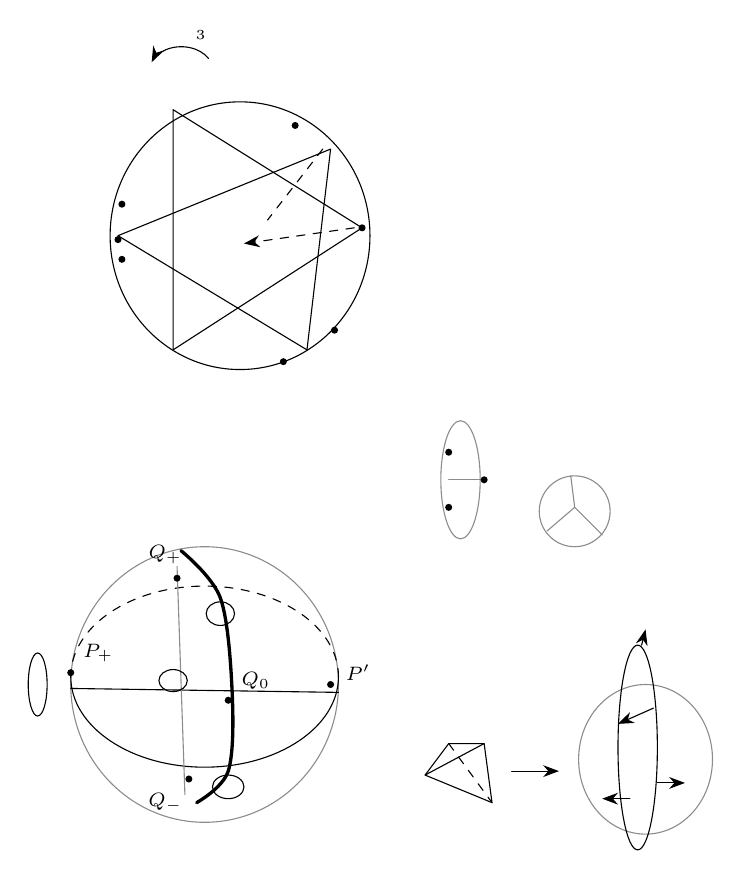
\begin{tikzpicture}[x=1mm,y=1mm,line cap=round,line join=round,font=\scriptsize]
\draw (26.5,-32) ellipse[x radius=16.5, y radius=17];
\draw (18,-16) -- (42,-31) -- (18,-46.5) -- cycle;
\draw (11,-32) -- (38,-21) -- (35,-46.5) -- cycle;
\draw[dashed] (37,-21) -- (30,-30);
\draw[dashed,-{Stealth[length=2mm]}] (41,-31) -- (27,-33);
\node[pt] at (33.5,-18) {};
\node[pt] at (11.5,-28) {};
\node[pt] at (11,-32.5) {};
\node[pt] at (11.5,-35) {};
\node[pt] at (38.5,-44) {};
\node[pt] at (32,-48) {};
\node[pt] at (42,-31) {};
\draw[-{Stealth[length=2mm]}] (22.5,-9.5) arc[start angle=30, end angle=160, x radius=4, y radius=3];
\node[inner sep=1pt] at (21.5,-6.5) {\tiny $3$};
\draw[pencil] (22,-89) ellipse[x radius=17, y radius=17.5];
\draw[dashed] (39,-88) arc[start angle=0, end angle=180, x radius=17, y radius=11.5];
\draw (5,-88) arc[start angle=180, end angle=360, x radius=17, y radius=11.5];
\draw (5,-89.5) -- (39,-90);
\draw[very thick] plot[smooth, tension=0.55] coordinates {(19,-72) (24,-78) (25.5,-90) (25,-100) (21,-104)};
\draw[pencil] (18.5,-74) -- (19.5,-103);
\node[pt] at (18.5,-75.5) {};
\node[pt] at (20,-101) {};
\node[pt] at (5,-87.5) {};
\node[pt] at (25,-91) {};
\node[pt] at (38,-89) {};
\node[inner sep=1pt] at (17,-72.5) {\scriptsize $Q_+$};
\node[inner sep=1pt] at (17,-104) {\scriptsize $Q_-$};
\node[inner sep=1pt] at (8.5,-85) {\scriptsize $P_+$};
\node[inner sep=1pt] at (28.5,-88.5) {\scriptsize $Q_0$};
\node[inner sep=1pt] at (41.5,-87.5) {\scriptsize $P'$};
\draw (24,-80) ellipse[x radius=1.8, y radius=1.5];
\draw (18,-88.5) ellipse[x radius=1.8, y radius=1.4];
\draw (25,-102) ellipse[x radius=2, y radius=1.5];
\draw (0.8,-89) ellipse[x radius=1.2, y radius=4];
\draw[pencil] (54.5,-63) ellipse[x radius=2.5, y radius=7.5];
\draw[pencil] (53,-63) -- (57.5,-63);
\node[pt] at (53,-59.5) {};
\node[pt] at (57.5,-63) {};
\node[pt] at (53,-66.5) {};
\draw[pencil] (69,-67) circle[radius=4.5];
\draw[pencil] (69,-66.5) -- (68.5,-62.5);
\draw[pencil] (69,-66.5) -- (65.5,-69.5);
\draw[pencil] (69,-66.5) -- (72.5,-70);
\draw (50,-100.5) -- (53,-96.5) -- (57.5,-96.5) -- (58.5,-104) -- cycle;
\draw (50,-100.5) -- (57.5,-96.5);
\draw[dashed] (53,-96.5) -- (58.5,-104);
\draw[-{Stealth[length=2mm]}] (61,-100) -- (67,-100);
\draw[pencil] (78,-98.5) ellipse[x radius=8.5, y radius=9.5];
\draw (77,-97) ellipse[x radius=2.5, y radius=13];
\draw[-{Stealth[length=2mm]}] (77.5,-84) -- (78,-82);
\draw[-{Stealth[length=2mm]}] (79,-92) -- (74.5,-94);
\draw[-{Stealth[length=2mm]}] (79.5,-101.5) -- (83,-101.5);
\draw[-{Stealth[length=2mm]}] (76,-103.5) -- (72.5,-103.5);
\end{tikzpicture}
\end{document}
